%% This file was auto-generated by IPython.
%% Conversion from the original notebook file:
%% Exercise 10.ipynb
%%
\documentclass[11pt,english]{article}

%% This is the automatic preamble used by IPython.  Note that it does *not*
%% include a documentclass declaration. The documentclass is added at runtime
%% to the overall document.
\usepackage{fancyhdr}
\usepackage{amsmath}
\usepackage{amssymb}
\usepackage{graphicx}
\usepackage{ucs}
\usepackage[utf8x]{inputenc}

% needed for markdown enumerations to work
\usepackage{enumerate}

% Slightly bigger margins than the latex defaults
\usepackage{geometry}
\geometry{verbose,tmargin=3cm,bmargin=3cm,lmargin=2.5cm,rmargin=2.5cm}

% Define a few colors for use in code, links and cell shading
\usepackage{color}
\definecolor{orange}{cmyk}{0,0.4,0.8,0.2}
\definecolor{darkorange}{rgb}{.71,0.21,0.01}
\definecolor{darkgreen}{rgb}{.12,.54,.11}
\definecolor{myteal}{rgb}{.26, .44, .56}
\definecolor{gray}{gray}{0.45}
\definecolor{lightgray}{gray}{.95}
\definecolor{mediumgray}{gray}{.8}
\definecolor{inputbackground}{rgb}{.95, .95, .85}
\definecolor{outputbackground}{rgb}{.95, .95, .95}
\definecolor{traceback}{rgb}{1, .95, .95}

% Framed environments for code cells (inputs, outputs, errors, ...).  The
% various uses of \unskip (or not) at the end were fine-tuned by hand, so don't
% randomly change them unless you're sure of the effect it will have.
\usepackage{framed}

% remove extraneous vertical space in boxes
\setlength\fboxsep{0pt}

% codecell is the whole input+output set of blocks that a Code cell can
% generate.

% TODO: unfortunately, it seems that using a framed codecell environment breaks
% the ability of the frames inside of it to be broken across pages.  This
% causes at least the problem of having lots of empty space at the bottom of
% pages as new frames are moved to the next page, and if a single frame is too
% long to fit on a page, it will completely stop latex from compiling the
% document.  So unless we figure out a solution to this, we'll have to instead
% leave the codecell env. as empty.  I'm keeping the original codecell
% definition here (a thin vertical bar) for reference, in case we find a
% solution to the page break issue.

%% \newenvironment{codecell}{%
%%     \def\FrameCommand{\color{mediumgray} \vrule width 1pt \hspace{5pt}}%
%%    \MakeFramed{\vspace{-0.5em}}}
%%  {\unskip\endMakeFramed}

% For now, make this a no-op...
\newenvironment{codecell}{}

 \newenvironment{codeinput}{%
   \def\FrameCommand{\colorbox{inputbackground}}%
   \MakeFramed{\advance\hsize-\width \FrameRestore}}
 {\unskip\endMakeFramed}

\newenvironment{codeoutput}{%
   \def\FrameCommand{\colorbox{outputbackground}}%
   \vspace{-1.4em}
   \MakeFramed{\advance\hsize-\width \FrameRestore}}
 {\unskip\medskip\endMakeFramed}

\newenvironment{traceback}{%
   \def\FrameCommand{\colorbox{traceback}}%
   \MakeFramed{\advance\hsize-\width \FrameRestore}}
 {\endMakeFramed}

% Use and configure listings package for nicely formatted code
\usepackage{listingsutf8}
\lstset{
  language=python,
  inputencoding=utf8x,
  extendedchars=\true,
  aboveskip=\smallskipamount,
  belowskip=\smallskipamount,
  xleftmargin=2mm,
  breaklines=true,
  basicstyle=\small \ttfamily,
  showstringspaces=false,
  keywordstyle=\color{blue}\bfseries,
  commentstyle=\color{myteal},
  stringstyle=\color{darkgreen},
  identifierstyle=\color{darkorange},
  columns=fullflexible,  % tighter character kerning, like verb
}

% The hyperref package gives us a pdf with properly built
% internal navigation ('pdf bookmarks' for the table of contents,
% internal cross-reference links, web links for URLs, etc.)
\usepackage{hyperref}
\hypersetup{
  breaklinks=true,  % so long urls are correctly broken across lines
  colorlinks=true,
  urlcolor=blue,
  linkcolor=darkorange,
  citecolor=darkgreen,
  }

% hardcode size of all verbatim environments to be a bit smaller
\makeatletter
\g@addto@macro\@verbatim\small\topsep=0.5em\partopsep=0pt
\makeatother

% Prevent overflowing lines due to urls and other hard-to-break entities.
\sloppy

\newcommand{\HRule}{\rule{\linewidth}{0.5mm}}
\title{\bf K-means, hierarchical, and “soft” clustering}
\author{Xugang Zhou \\ Fangzhou Yang}
\pagestyle{fancy}
\lhead{{\bf Machine Intelligence 2 SS2013}}
\rhead{Exercise 10}
\renewcommand{\headrulewidth}{0.4pt}

\begin{document}
\begin{titlepage}
\begin{center}
\vfill
\textsc{\LARGE Machine Intelligence 2}\\[1.5cm]
\textsc{\Large Exercise 10}\\[0.5cm]

\HRule \\[0.4cm]
{\huge \bfseries K-means, hierarchical, and “soft” clustering}\\[0.4cm]
\HRule \\[1.5cm]
\begin{minipage}{0.4\textwidth}
\begin{flushleft} \large
\emph{Group Members:}\\
Xugang \textsc{Zhou}\\
Fangzhou \textsc{Yang}
\end{flushleft}
\end{minipage}
\begin{minipage}{0.4\textwidth}
\begin{flushright} \large
\emph{Tutor:} \\
Timm \textsc{Lochmann} \\
\end{flushright}
\end{minipage}
\vfill
{\large \today}\\
\end{center}
\end{titlepage}
\thispagestyle{fancy}

\section{10.1 K-means and hierarchical clustering}

\begin{codecell}
\begin{codeinput}
\begin{lstlisting}
#function
from numpy import *
import matplotlib
import matplotlib.pyplot as plt
import cluster
from mpl_toolkits.mplot3d import Axes3D

def plot3dScatter(X,Y,Z,title,c):
    fig = plt.figure()
    ax = Axes3D(fig)
    ax.plot(X,Y,Z,c)
    ax.set_title(title)
    plt.show()

def plotScatter(X,Y,title,c,ran):
    fig = plt.figure()
    ax = fig.add_subplot(111)
    ax.axis([-ran,ran,-ran,ran])
    ax.plot(X,Y,c+'.')
    ax.set_title(title)
    plt.show()
    
def plotScatter2(X,Y,title):
    fig = plt.figure()
    ax = fig.add_subplot(111)
    for i in range (len(X)):
        ax.plot(X[i],Y[i],'g.')
    ax.set_title(title)
    plt.show()
    
def plotCluster(clusters,colors,title,ran):
    fig = plt.figure()
    ax = fig.add_subplot(111)
    ax.axis([-ran,ran,-ran,ran])
    for i in range (len(clusters)):
        for j in range (len(clusters[i])):
            ax.plot(clusters[i][j][0],clusters[i][j][1],colors[i]+'.')
    ax.set_title(title)
    plt.show()
    
    
def plotCluster3d(X,Y,Z,result,colors,title):
    fig = plt.figure()
    ax = Axes3D(fig)
    for i in range (len(X)):
        ax.scatter(X[i],Y[i],Z[i],c=colors[result[i]-1] )
    ax.set_title(title)
    plt.show()
\end{lstlisting}
\end{codeinput}
\end{codecell}
\subsection{stripes2}

\begin{codecell}
\begin{codeinput}
\begin{lstlisting}
data = loadtxt("clusters/stripes2.csv",skiprows=1,delimiter=",",usecols=(1,2))
X = data[:,0]
Y = data[:,1]
plotScatter(X,Y,"Scatter Plot of stripes",'g',3)

kdata = [0 for i in range (len(X))]
for i in range (len(X)):
    kdata[i] = (X[i],Y[i])
    
\end{lstlisting}
\end{codeinput}
\begin{codeoutput}
\begin{center}
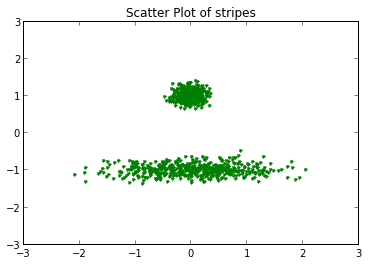
\includegraphics[width=0.7\textwidth]{Exercise_10_files/Exercise_10_fig_00.png}
\par
\end{center}
\end{codeoutput}
\end{codecell}
\begin{codecell}
\begin{codeinput}
\begin{lstlisting}
#Kmeans
cl = cluster.KMeansClustering(kdata)
result = cl.getclusters(2)
\end{lstlisting}
\end{codeinput}
\end{codecell}
\begin{codecell}
\begin{codeinput}
\begin{lstlisting}
colors = ['r','g','b','c','m']
plotCluster(result,colors,"KMeans Clustering of Dataset-stripes2",3)
\end{lstlisting}
\end{codeinput}
\begin{codeoutput}
\begin{center}
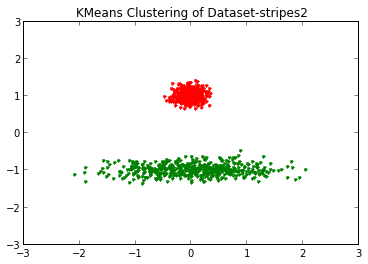
\includegraphics[width=0.7\textwidth]{Exercise_10_files/Exercise_10_fig_01.png}
\par
\end{center}
\end{codeoutput}
\end{codecell}
\subsection{Ring}

\begin{codecell}
\begin{codeinput}
\begin{lstlisting}
data = loadtxt("clusters/ring.csv",skiprows=1,delimiter=",",usecols=(1,2))
X = data[:,0]
Y = data[:,1]
plotScatter(X,Y,"Scatter Plot of Ring",'g',3)

kdata = [0 for i in range (len(X))]
for i in range (len(X)):
    kdata[i] = (X[i],Y[i])
\end{lstlisting}
\end{codeinput}
\begin{codeoutput}
\begin{center}
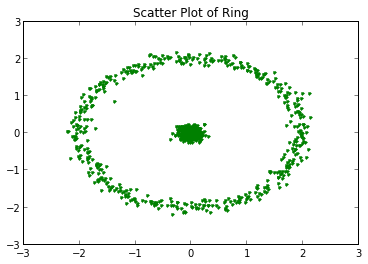
\includegraphics[width=0.7\textwidth]{Exercise_10_files/Exercise_10_fig_02.png}
\par
\end{center}
\end{codeoutput}
\end{codecell}
\begin{codecell}
\begin{codeinput}
\begin{lstlisting}
#Kmeans
cl = cluster.KMeansClustering(kdata)
result = cl.getclusters(2)
\end{lstlisting}
\end{codeinput}
\end{codecell}
\begin{codecell}
\begin{codeinput}
\begin{lstlisting}
colors = ['r','g','b','c','m']
plotCluster(result,colors,"KMeans Clustering of Dataset-Ring",3)
\end{lstlisting}
\end{codeinput}
\begin{codeoutput}
\begin{center}
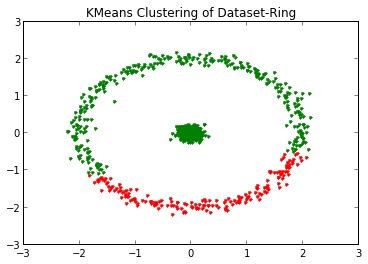
\includegraphics[width=0.7\textwidth]{Exercise_10_files/Exercise_10_fig_03.png}
\par
\end{center}
\end{codeoutput}
\end{codecell}
\begin{codecell}
\begin{codeinput}
\begin{lstlisting}
#Single-Linkage
cl = cluster.HierarchicalClustering(kdata, lambda (x1,y1),(x2,y2): math.sqrt((x1-x2)**2+(y1-y2)**2),'single' )
result = cl.getlevel(1)


\end{lstlisting}
\end{codeinput}
\end{codecell}
\begin{codecell}
\begin{codeinput}
\begin{lstlisting}
colors = ['r','g','b','c','m']
plotCluster(result,colors,"Single-Linkage Clustering of Dataset-Ring",3)
\end{lstlisting}
\end{codeinput}
\begin{codeoutput}
\begin{center}
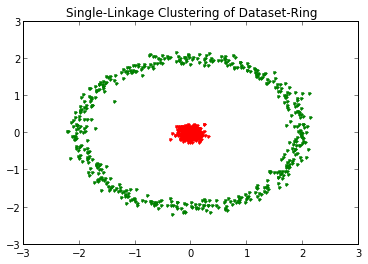
\includegraphics[width=0.7\textwidth]{Exercise_10_files/Exercise_10_fig_04.png}
\par
\end{center}
\end{codeoutput}
\end{codecell}
\subsection{stripes3}

\begin{codecell}
\begin{codeinput}
\begin{lstlisting}
data = loadtxt("clusters/stripes3.csv",skiprows=1,delimiter=",",usecols=(1,2))
X = data[:,0]
Y = data[:,1]
plotScatter(X,Y,"Scatter Plot of stripes3",'g',3)

kdata = [0 for i in range (len(X))]
for i in range (len(X)):
    kdata[i] = (X[i],Y[i])
\end{lstlisting}
\end{codeinput}
\begin{codeoutput}
\begin{center}
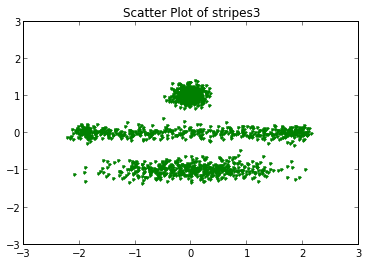
\includegraphics[width=0.7\textwidth]{Exercise_10_files/Exercise_10_fig_05.png}
\par
\end{center}
\end{codeoutput}
\end{codecell}
\begin{codecell}
\begin{codeinput}
\begin{lstlisting}
#Kmeans
cl = cluster.KMeansClustering(kdata)
result = cl.getclusters(2)
\end{lstlisting}
\end{codeinput}
\end{codecell}
\begin{codecell}
\begin{codeinput}
\begin{lstlisting}
colors = ['r','g','b','c','m']
plotCluster(result,colors,"KMeans Clustering of Dataset-stripes3",3)
\end{lstlisting}
\end{codeinput}
\begin{codeoutput}
\begin{center}
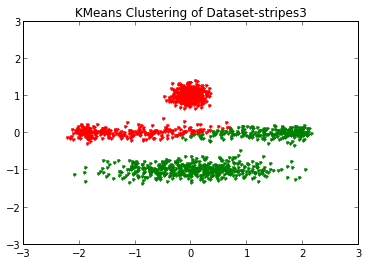
\includegraphics[width=0.7\textwidth]{Exercise_10_files/Exercise_10_fig_06.png}
\par
\end{center}
\end{codeoutput}
\end{codecell}
\begin{codecell}
\begin{codeinput}
\begin{lstlisting}
#Single-Linkage
cl = cluster.HierarchicalClustering(kdata, lambda (x1,y1),(x2,y2): math.sqrt((x1-x2)**2+(y1-y2)**2),'single' )
result = cl.getlevel(0.3)
\end{lstlisting}
\end{codeinput}
\end{codecell}
\begin{codecell}
\begin{codeinput}
\begin{lstlisting}
colors = ['r','g','b','c','m']
plotCluster(result,colors,"Single-Linkage Clustering of Dataset-stripes3",3)
\end{lstlisting}
\end{codeinput}
\begin{codeoutput}
\begin{center}
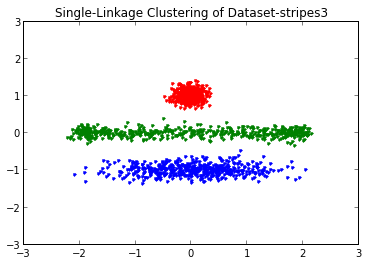
\includegraphics[width=0.7\textwidth]{Exercise_10_files/Exercise_10_fig_07.png}
\par
\end{center}
\end{codeoutput}
\end{codecell}
\begin{codecell}
\begin{codeinput}
\begin{lstlisting}
#linkage
import scipy.cluster.hierarchy as ch

kdata = [[0 for j in range (2)] for i in range (len(X))]
for i in range (len(X)):
    kdata[i][0] = X[i]
    kdata[i][1] = Y[i]

dis = scipy.spatial.distance.pdist(matrix(kdata))

linkresult = ch.linkage(dis)
den = ch.dendrogram(linkresult,get_leaves=False,show_leaf_counts=False)
\end{lstlisting}
\end{codeinput}
\begin{codeoutput}
\begin{center}
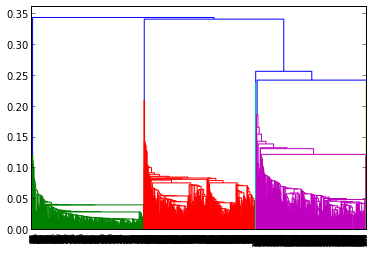
\includegraphics[width=0.7\textwidth]{Exercise_10_files/Exercise_10_fig_08.png}
\par
\end{center}
\end{codeoutput}
\end{codecell}
\subsection{3d}

\begin{codecell}
\begin{codeinput}
\begin{lstlisting}
data = loadtxt("clusters/3d.csv",skiprows=1,delimiter=",",usecols=(1,2,3))
X = data[:,0]
Y = data[:,1]
Z = data[:,2]
plot3dScatter(X,Y,Z,"Scatter Plot of 3d",'g.')

kdata = [0 for i in range (len(X))]
for i in range (len(X)):
    kdata[i] = (X[i],Y[i],Z[i])
\end{lstlisting}
\end{codeinput}
\begin{codeoutput}
\begin{center}
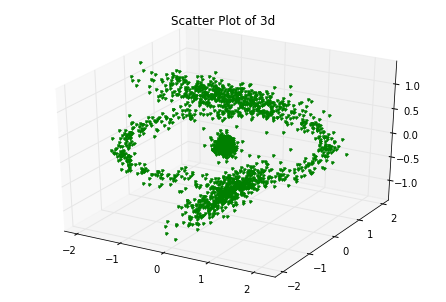
\includegraphics[width=0.7\textwidth]{Exercise_10_files/Exercise_10_fig_09.png}
\par
\end{center}
\end{codeoutput}
\end{codecell}
\begin{codecell}
\begin{codeinput}
\begin{lstlisting}
#linkage
import scipy.cluster.hierarchy as ch

hdata = [[0 for j in range (3)] for i in range (len(X))]
for i in range (len(X)):
    hdata[i][0] = X[i]
    hdata[i][1] = Y[i]
    hdata[i][2] = Z[i]

dis = scipy.spatial.distance.pdist(matrix(hdata))

linkresult = ch.linkage(dis)
den = ch.dendrogram(linkresult,get_leaves=False,show_leaf_counts=False)

\end{lstlisting}
\end{codeinput}
\begin{codeoutput}
\begin{center}
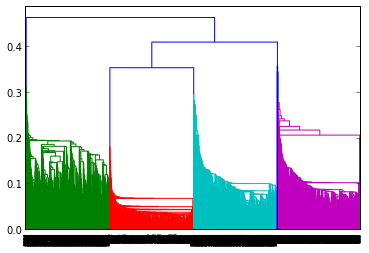
\includegraphics[width=0.7\textwidth]{Exercise_10_files/Exercise_10_fig_10.png}
\par
\end{center}
\end{codeoutput}
\end{codecell}
\begin{codecell}
\begin{codeinput}
\begin{lstlisting}
R = ch.fcluster(linkresult,t=0.35,criterion='distance')
\end{lstlisting}
\end{codeinput}
\end{codecell}
\begin{codecell}
\begin{codeinput}
\begin{lstlisting}
colors = ['r','g','b','c','m']
plotCluster3d(X,Y,Z,R,colors,"Clustering of Dataset-3d")
\end{lstlisting}
\end{codeinput}
\begin{codeoutput}
\begin{center}
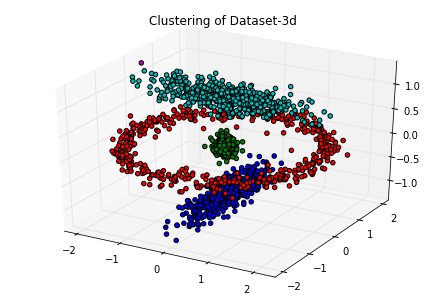
\includegraphics[width=0.7\textwidth]{Exercise_10_files/Exercise_10_fig_11.png}
\par
\end{center}
\end{codeoutput}
\end{codecell}
\section{10.2 Soft K-means Clustering}

\begin{codecell}
\begin{codeinput}
\begin{lstlisting}
#init W
def init_w(k,rSeed):
    random.seed(rSeed)
    W_init = [[0 for j in range(2)] for i in range(k)]
    for p in range(k):
        W_init[p][0] = random.random() * 6 - 3
        W_init[p][1] = random.random() * 6 -3
    return W_init

\end{lstlisting}
\end{codeinput}
\end{codecell}
\begin{codecell}
\begin{codeinput}
\begin{lstlisting}
#soft-Kmeans
def kmeans_soft(X,Y,k,gamma,W_init,beta0,ita,betaf):
    beta = beta0
    W = [[ W_init[i][j] for j in range (len(W_init[0])) ] for i in range (len(W_init)) ]
    W_new = [[ W_init[i][j] for j in range (len(W_init[0])) ] for i in range (len(W_init))]
    m = [[0 for j in range(k)] for i in range(len(X))] 
    
    while True:
    
        end = False
        while True:
            for alpha in range (len(X)):
                tmpSum = 0.
                for q in range (k):
                    tmpSum += math.exp(-beta/2 * ( (X[alpha] - W[q][0])**2 + (Y[alpha] - W[q][1])**2 ) )
                for p in range (k):
                    m[alpha][p] = math.exp(-beta/2 * ( (X[alpha] - W[p][0])**2 + (Y[alpha] - W[p][1])**2 ) ) / tmpSum
            for p in range (k):
                mx_sum = 0.
                my_sum = 0.
                m_sum = 0.
                for alpha in range (len(X)):
                    mx_sum += m[alpha][p] * X[alpha]
                    my_sum += m[alpha][p] * Y[alpha]
                    m_sum += m[alpha][p]
                W_new[p][0] = mx_sum / m_sum
                W_new[p][1] = my_sum / m_sum
                
            count = 0
            for q in range(k):
                if( math.sqrt( (W_new[q][0] - W[q][0])**2 + (W_new[q][1] - W[q][1])**2 ) < gamma):
                    count += 1
            if(count == k):
                end = True
            
            W = W_new[:][:]
            
            if (end):
                break
        
        beta = ita * beta
        if(beta > betaf):
            break
        
    return W,m
\end{lstlisting}
\end{codeinput}
\end{codecell}
\begin{codecell}
\begin{codeinput}
\begin{lstlisting}
def plotCluster(X,Y,title,colors,ran,m, W):
    fig = plt.figure()
    ax = fig.add_subplot(111)
    ax.axis([-ran,ran,-ran,ran])
    for i in range (len(X)):
        #find the max probability
        for q in range (k):
            if(q == 0):
                m_max = m[i][q]
                p = q
            else:
                if(m_max < m[i][q]):
                    m_max = m[i][q]
                    p = q
        ax.plot(X[i],Y[i],colors[p]+'.')
    for i in range (len(W)):
        ax.plot(W[i][0],W[i][1],colors[i]+'D')
        ax.plot(W[i][0],W[i][1],'y'+'H')
    ax.set_title(title)
    plt.show()
\end{lstlisting}
\end{codeinput}
\end{codecell}
\begin{codecell}
\begin{codeinput}
\begin{lstlisting}
def assignPoint(W,x,y):
    k = len(W)
    for i in range(k):
        if(i==0):
            min_distance = distance(W[i][0],W[i][1],x,y)
            min_p = i
        else:
            d = distance(W[i][0],W[i][1],x,y)
            if(d < min_distance):
                min_distance = d
                min_p = i
    return min_p

def drawBoundary(X,Y,title,ran, W_init, W, fine):
    fig = plt.figure()
    ax = fig.add_subplot(111)
    ax.axis([-ran,ran,-ran,ran])
    
    ax.plot(X,Y,'g'+'.')
    
    for i in range (len(W_init)):
        ax.plot(W_init[i][0],W_init[i][1],'r'+'H')
    
    for i in range (len(W)):
        ax.plot(W[i][0],W[i][1],'k'+'H')
        
    ax.set_title(title)
    
    ran = float(ran)
    unit = 2*ran/fine
    print 'unit',unit
    for i in range(fine):
        x = -ran + i*unit
        for j in range(fine):
            y = -ran + j*unit
            #print x,y
            p0 = assignPoint(W,x,y)
            p1 = assignPoint(W,x+unit,y)
            p2 = assignPoint(W,x-unit,y)
            p3 = assignPoint(W,x,y+unit)
            p4 = assignPoint(W,x,y-unit)
            if(p0==p1 and p1==p2 and p2==p3 and p3==p4):
                continue
            else:
                ax.plot(x,y,'y.')
    plt.show()
\end{lstlisting}
\end{codeinput}
\end{codecell}
\begin{codecell}
\begin{codeinput}
\begin{lstlisting}
#read data
data = loadtxt("cluster.dat")
print data.shape

X = data[0,:]
Y = data[1,:]

plotScatter(X,Y,"Scatter Plot", 'g', 3)
\end{lstlisting}
\end{codeinput}
\begin{codeoutput}
\begin{verbatim}
(2, 500)
\end{verbatim}
\begin{center}
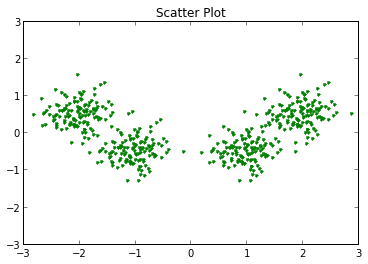
\includegraphics[width=0.7\textwidth]{Exercise_10_files/Exercise_10_fig_12.png}
\par
\end{center}
\end{codeoutput}
\end{codecell}
\subsection{Non-Annealing}

\begin{codecell}
\begin{codeinput}
\begin{lstlisting}
k = 8
rSeed = 100
W_init = init_w(k,rSeed)
print "W_init"
print matrix(W_init)
gamma = 0.01
ita = 1.1
W_result = [ W_init[:][:] for i in range (100)]
m_result = [ m[:][:] for i in range (100)]
for t in range(100):
    beta0 = 0.2 * (t+1)
    betaf = beta0
    W_return , m_return = kmeans_soft(X,Y,k,gamma,W_init,beta0,ita,betaf)
    W_result[t] = W_return[:][:]
    m_result[t] = m_return[:][:]
    if(t<10 or t%10==0):
        W_plot = W_result[t][:][:]
        drawBoundary(X,Y,"Boundary(beta="+str(beta0)+")",3, W_init, W_plot, 100)
\end{lstlisting}
\end{codeinput}

\begin{codeoutput}
\begin{verbatim}
W_init
[[ 0.26042965 -1.32978369]
 [-0.45289446  2.06865679]
 [-2.97168686 -2.27058528]
 [ 1.02449451  1.95511653]
 [-2.17976046  0.45055998]
 [ 2.34793173 -1.74478727]
 [-1.88803068 -2.34973866]
 [-1.68181504  2.87174271]]
unit
\end{verbatim}
\begin{verbatim}
0.06
\end{verbatim}
\begin{center}
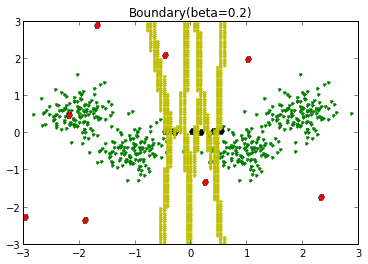
\includegraphics[width=0.7\textwidth]{Exercise_10_files/Exercise_10_fig_13.png}
\par
\end{center}
\begin{verbatim}
unit 0.06
\end{verbatim}
\begin{center}
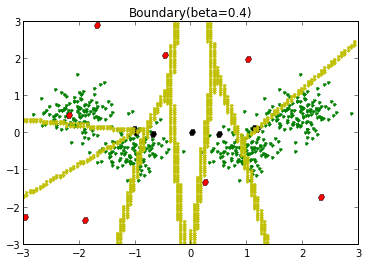
\includegraphics[width=0.7\textwidth]{Exercise_10_files/Exercise_10_fig_14.png}
\par
\end{center}
\begin{verbatim}
unit 0.06
\end{verbatim}
\begin{center}
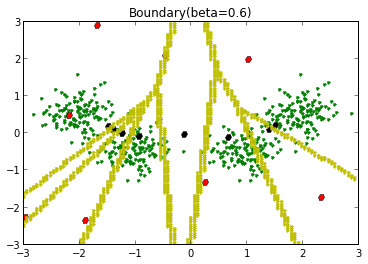
\includegraphics[width=0.7\textwidth]{Exercise_10_files/Exercise_10_fig_15.png}
\par
\end{center}
\begin{verbatim}
unit 0.06
\end{verbatim}
\begin{center}
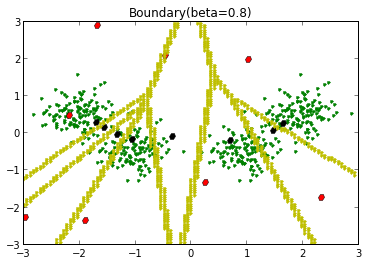
\includegraphics[width=0.7\textwidth]{Exercise_10_files/Exercise_10_fig_16.png}
\par
\end{center}
\begin{verbatim}
unit 0.06
\end{verbatim}
\begin{center}
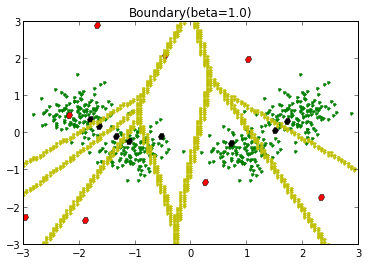
\includegraphics[width=0.7\textwidth]{Exercise_10_files/Exercise_10_fig_17.png}
\par
\end{center}
\begin{verbatim}
unit 0.06
\end{verbatim}
\begin{center}
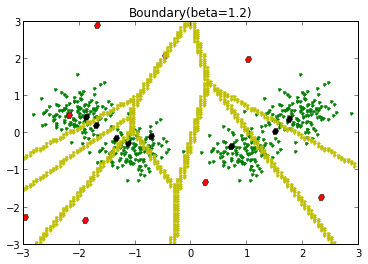
\includegraphics[width=0.7\textwidth]{Exercise_10_files/Exercise_10_fig_18.png}
\par
\end{center}
\begin{verbatim}
unit 0.06
\end{verbatim}
\begin{center}
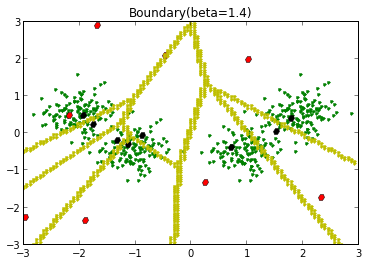
\includegraphics[width=0.7\textwidth]{Exercise_10_files/Exercise_10_fig_19.png}
\par
\end{center}
\begin{verbatim}
unit 0.06
\end{verbatim}
\begin{center}
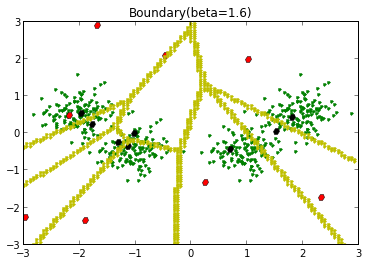
\includegraphics[width=0.7\textwidth]{Exercise_10_files/Exercise_10_fig_20.png}
\par
\end{center}
\begin{verbatim}
unit 0.06
\end{verbatim}
\begin{center}
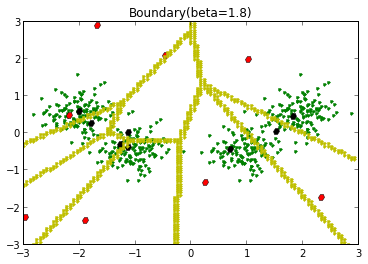
\includegraphics[width=0.7\textwidth]{Exercise_10_files/Exercise_10_fig_21.png}
\par
\end{center}
\begin{verbatim}
unit 0.06
\end{verbatim}
\begin{center}
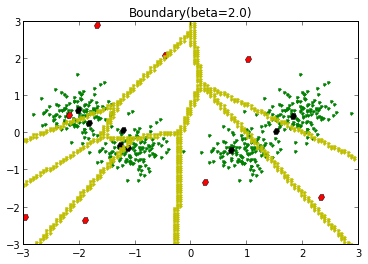
\includegraphics[width=0.7\textwidth]{Exercise_10_files/Exercise_10_fig_22.png}
\par
\end{center}
\begin{verbatim}
unit 0.06
\end{verbatim}
\begin{center}
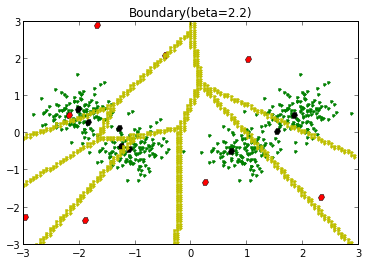
\includegraphics[width=0.7\textwidth]{Exercise_10_files/Exercise_10_fig_23.png}
\par
\end{center}
\begin{verbatim}
unit 0.06
\end{verbatim}
\begin{center}
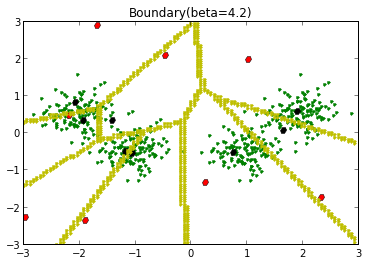
\includegraphics[width=0.7\textwidth]{Exercise_10_files/Exercise_10_fig_24.png}
\par
\end{center}
\begin{verbatim}
unit 0.06
\end{verbatim}
\begin{center}
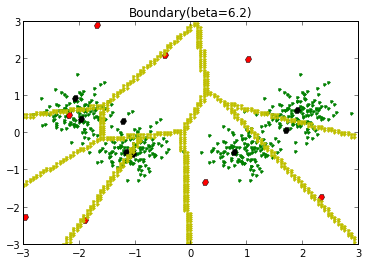
\includegraphics[width=0.7\textwidth]{Exercise_10_files/Exercise_10_fig_25.png}
\par
\end{center}
\begin{verbatim}
unit 0.06
\end{verbatim}
\begin{center}
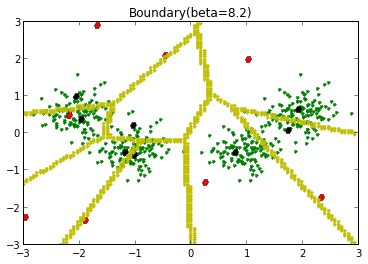
\includegraphics[width=0.7\textwidth]{Exercise_10_files/Exercise_10_fig_26.png}
\par
\end{center}
\begin{verbatim}
unit 0.06
\end{verbatim}
\begin{center}
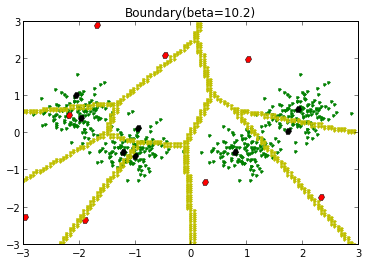
\includegraphics[width=0.7\textwidth]{Exercise_10_files/Exercise_10_fig_27.png}
\par
\end{center}
\begin{verbatim}
unit 0.06
\end{verbatim}
\begin{center}
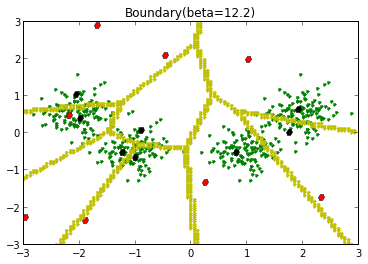
\includegraphics[width=0.7\textwidth]{Exercise_10_files/Exercise_10_fig_28.png}
\par
\end{center}
\begin{verbatim}
unit 0.06
\end{verbatim}
\begin{center}
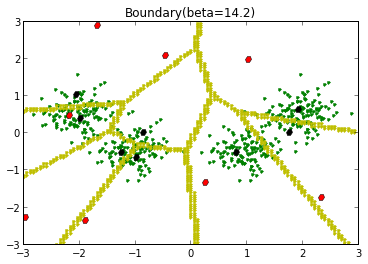
\includegraphics[width=0.7\textwidth]{Exercise_10_files/Exercise_10_fig_29.png}
\par
\end{center}
\begin{verbatim}
unit 0.06
\end{verbatim}
\begin{center}
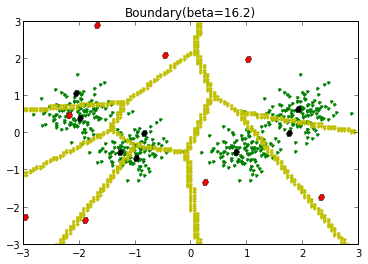
\includegraphics[width=0.7\textwidth]{Exercise_10_files/Exercise_10_fig_30.png}
\par
\end{center}
\begin{verbatim}
unit 0.06
\end{verbatim}
\begin{center}
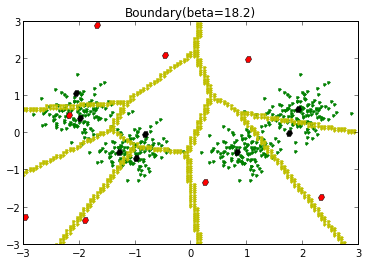
\includegraphics[width=0.7\textwidth]{Exercise_10_files/Exercise_10_fig_31.png}
\par
\end{center}
\end{codeoutput}
\end{codecell}
\begin{codecell}
\begin{codeinput}
\begin{lstlisting}
#Plot the first coordinates of the final prototypes against the beta
W_first_x = [0 for i in range (100)]
W_first_y = [0 for i in range (100)]
for t in range(100):
    beta0 = 0.2 * (t+1)
    W_first_x[t] = W_result[t][0][0]
    W_first_y[t] = W_result[t][0][1]
plotScatter2(W_first_x[:], W_first_y[:], "the first coordinates of the final prototypes against the beta")
\end{lstlisting}
\end{codeinput}
\begin{codeoutput}
\begin{center}
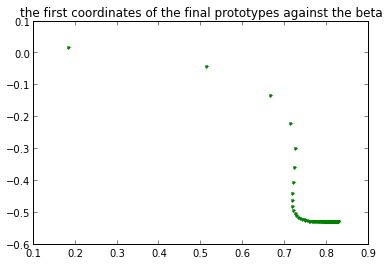
\includegraphics[width=0.7\textwidth]{Exercise_10_files/Exercise_10_fig_32.png}
\par
\end{center}
\end{codeoutput}
\end{codecell}
\subsection{Annealing}

\begin{codecell}
\begin{codeinput}
\begin{lstlisting}
k_array = [ 4, 6, 8 ]
rSeed = 100

gamma = 0.01
ita = 1.1
beta0 = 0.2
betaf = 20


W_result2 = [ W_init[:][:] for i in range (len(k_array))]
m_result2 = [ m[:][:] for i in range (len(k_array))]

for t in range(len(k_array)):
    W_init = init_w(k_array[t],rSeed)
    W_return , m_return = kmeans_soft(X,Y,k_array[t],gamma,W_init,beta0,ita,betaf)
    W_result[t] = W_return[:][:]
    m_result[t] = m_return[:][:]
    W_plot = W_result[t][:][:]
    drawBoundary(X,Y,"Boundary(K="+str(k_array[t])+")",3, W_init, W_plot, 100)

\end{lstlisting}
\end{codeinput}
\begin{codeoutput}
\begin{verbatim}
unit 0.06
\end{verbatim}
\begin{center}
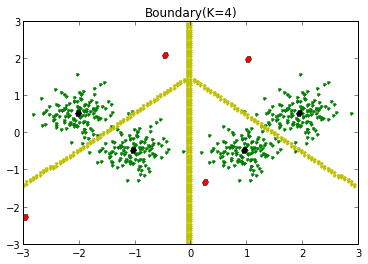
\includegraphics[width=0.7\textwidth]{Exercise_10_files/Exercise_10_fig_33.png}
\par
\end{center}
\begin{verbatim}
unit 0.06
\end{verbatim}
\begin{center}
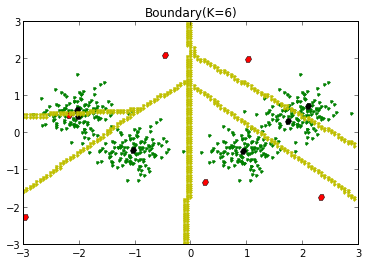
\includegraphics[width=0.7\textwidth]{Exercise_10_files/Exercise_10_fig_34.png}
\par
\end{center}
\begin{verbatim}
unit 0.06
\end{verbatim}
\begin{center}
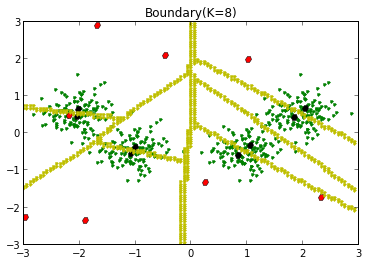
\includegraphics[width=0.7\textwidth]{Exercise_10_files/Exercise_10_fig_35.png}
\par
\end{center}
\end{codeoutput}
\end{codecell}

\end{document}
